% Options for packages loaded elsewhere
\PassOptionsToPackage{unicode}{hyperref}
\PassOptionsToPackage{hyphens}{url}
\PassOptionsToPackage{dvipsnames,svgnames,x11names}{xcolor}
%
\documentclass[
]{krantz}
\usepackage{amsmath,amssymb}
\usepackage{iftex}
\ifPDFTeX
  \usepackage[T1]{fontenc}
  \usepackage[utf8]{inputenc}
  \usepackage{textcomp} % provide euro and other symbols
\else % if luatex or xetex
  \usepackage{unicode-math} % this also loads fontspec
  \defaultfontfeatures{Scale=MatchLowercase}
  \defaultfontfeatures[\rmfamily]{Ligatures=TeX,Scale=1}
\fi
\usepackage{lmodern}
\ifPDFTeX\else
  % xetex/luatex font selection
\fi
% Use upquote if available, for straight quotes in verbatim environments
\IfFileExists{upquote.sty}{\usepackage{upquote}}{}
\IfFileExists{microtype.sty}{% use microtype if available
  \usepackage[]{microtype}
  \UseMicrotypeSet[protrusion]{basicmath} % disable protrusion for tt fonts
}{}
\makeatletter
\@ifundefined{KOMAClassName}{% if non-KOMA class
  \IfFileExists{parskip.sty}{%
    \usepackage{parskip}
  }{% else
    \setlength{\parindent}{0pt}
    \setlength{\parskip}{6pt plus 2pt minus 1pt}}
}{% if KOMA class
  \KOMAoptions{parskip=half}}
\makeatother
\usepackage{xcolor}
\usepackage{longtable,booktabs,array}
\usepackage{calc} % for calculating minipage widths
% Correct order of tables after \paragraph or \subparagraph
\usepackage{etoolbox}
\makeatletter
\patchcmd\longtable{\par}{\if@noskipsec\mbox{}\fi\par}{}{}
\makeatother
% Allow footnotes in longtable head/foot
\IfFileExists{footnotehyper.sty}{\usepackage{footnotehyper}}{\usepackage{footnote}}
\makesavenoteenv{longtable}
\usepackage{graphicx}
\makeatletter
\def\maxwidth{\ifdim\Gin@nat@width>\linewidth\linewidth\else\Gin@nat@width\fi}
\def\maxheight{\ifdim\Gin@nat@height>\textheight\textheight\else\Gin@nat@height\fi}
\makeatother
% Scale images if necessary, so that they will not overflow the page
% margins by default, and it is still possible to overwrite the defaults
% using explicit options in \includegraphics[width, height, ...]{}
\setkeys{Gin}{width=\maxwidth,height=\maxheight,keepaspectratio}
% Set default figure placement to htbp
\makeatletter
\def\fps@figure{htbp}
\makeatother
\setlength{\emergencystretch}{3em} % prevent overfull lines
\providecommand{\tightlist}{%
  \setlength{\itemsep}{0pt}\setlength{\parskip}{0pt}}
\setcounter{secnumdepth}{5}
\usepackage{booktabs}
\usepackage{longtable}
\usepackage{hyperref}
\usepackage[bf,singlelinecheck=off]{caption}
\usepackage{geometry}
\geometry{margin=1in}
\usepackage{graphicx}
\usepackage{enumitem}

\usepackage{framed,color}
\definecolor{shadecolor}{RGB}{248,248,248}

\renewcommand{\textfraction}{0.05}
\renewcommand{\topfraction}{0.8}
\renewcommand{\bottomfraction}{0.8}
\renewcommand{\floatpagefraction}{0.75}

\renewenvironment{quote}{\begin{VF}}{\end{VF}}
\let\oldhref\href
\renewcommand{\href}[2]{#2\footnote{\url{#1}}}

\makeatletter
\newenvironment{kframe}{%
\medskip{}
\setlength{\fboxsep}{.8em}
 \def\at@end@of@kframe{}%
 \ifinner\ifhmode%
  \def\at@end@of@kframe{\end{minipage}}%
  \begin{minipage}{\columnwidth}%
 \fi\fi%
 \def\FrameCommand##1{\hskip\@totalleftmargin \hskip-\fboxsep
 \colorbox{shadecolor}{##1}\hskip-\fboxsep
     % There is no \\@totalrightmargin, so:
     \hskip-\linewidth \hskip-\@totalleftmargin \hskip\columnwidth}%
 \MakeFramed {\advance\hsize-\width
   \@totalleftmargin\z@ \linewidth\hsize
   \@setminipage}}%
 {\par\unskip\endMakeFramed%
 \at@end@of@kframe}
\makeatother

\usepackage{makeidx}
\makeindex

\urlstyle{tt}

\usepackage{amsthm}
\makeatletter
\def\thm@space@setup{%
  \thm@preskip=8pt plus 2pt minus 4pt
  \thm@postskip=\thm@preskip
}
\makeatother

\frontmatter
\ifLuaTeX
  \usepackage{selnolig}  % disable illegal ligatures
\fi
\usepackage[]{natbib}
\bibliographystyle{apalike}
\usepackage{bookmark}
\IfFileExists{xurl.sty}{\usepackage{xurl}}{} % add URL line breaks if available
\urlstyle{same}
\hypersetup{
  pdftitle={Climate And Statistics},
  pdfauthor={Henri Funk, Alexander Sasse, Helmut Küchenhoff, Ralf Ludwig},
  colorlinks=true,
  linkcolor={Maroon},
  filecolor={Maroon},
  citecolor={Blue},
  urlcolor={Blue},
  pdfcreator={LaTeX via pandoc}}

\title{Climate And Statistics}
\author{Henri Funk, Alexander Sasse, Helmut Küchenhoff, Ralf Ludwig}
\date{2025-03-18}

\begin{document}
\maketitle

% you may need to leave a few empty pages before the dedication page

%\cleardoublepage\newpage\thispagestyle{empty}\null
%\cleardoublepage\newpage\thispagestyle{empty}\null
%\cleardoublepage\newpage
\thispagestyle{empty}

\begin{center}
\end{center}

\setlength{\abovedisplayskip}{-5pt}
\setlength{\abovedisplayshortskip}{-5pt}

{
\hypersetup{linkcolor=}
\setcounter{tocdepth}{0}
\tableofcontents
}
\chapter*{Preface}\label{preface}


\emph{Author: Henri Funk}

\begin{center}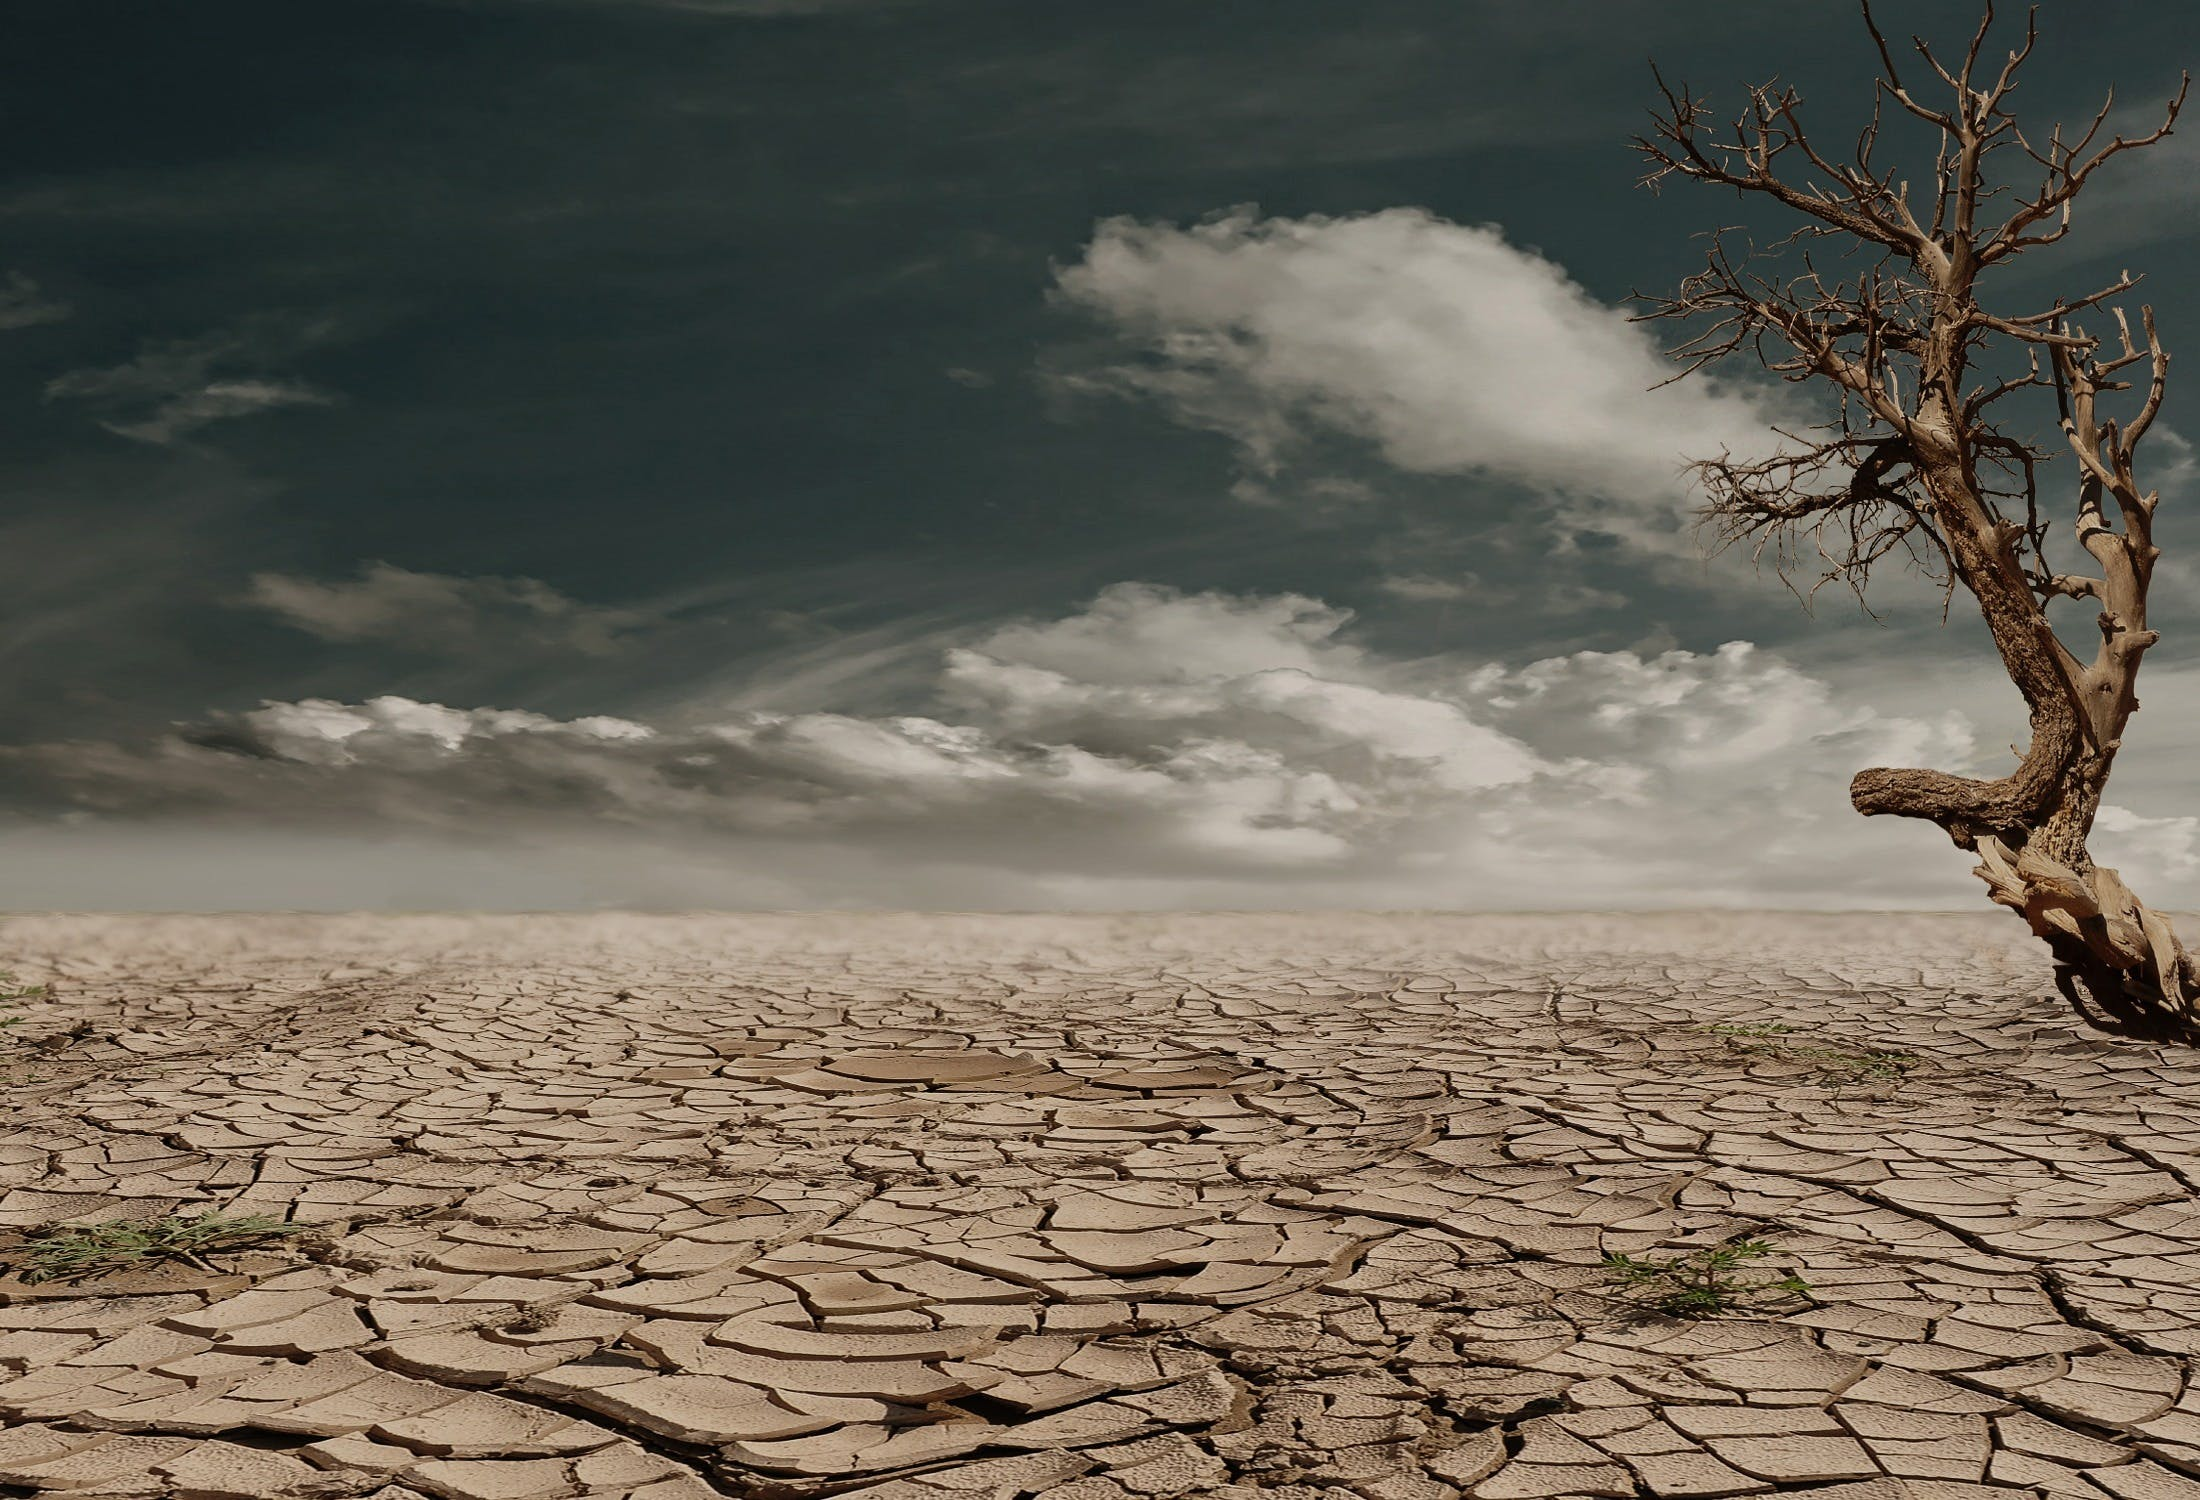
\includegraphics[width=0.75\linewidth]{cover} \end{center}

As the world faces the reality of climate change, natural hazards and extreme weather events have become a major concern, with devastating consequences for nature and humans. The quantification and definition of climate change, extreme events and its implications for life and health on our planet is one of the major concerns in climate science.

This book explains current statistical methods in climate science and their application.
We do not aim to provide a comprehensive overview of all statistical methods in climate science, but rather to give an overview of the most important methods and their application.
This book is the outcome of the seminar ``Climate and Statistics'' which took place in summer 2024 at the Department of Statistics, LMU Munich.

\begin{figure}
\centering

\includegraphics{by-nc-sa.png}
\caption{Creative Commons License}
\end{figure}

This book is licensed under the \href{http://creativecommons.org/licenses/by-nc-sa/4.0/}{Creative Commons Attribution-NonCommercial-ShareAlike 4.0 International License}.

\mainmatter

\section*{Technical Setup}\label{technical-setup}


The book chapters are written in the Markdown language.
To combine R-code and Markdown, we used rmarkdown.
The book was compiled with the bookdown package.
We collaborated using git and github.
For details, head over to the \href{https://github.com/henrifnk/Seminar_ClimateNStatistics}{book's repository}.

\chapter{Introduction}\label{introduction}

\emph{Author: }

\emph{Supervisor: }

\section{Intro About the Seminar Topic}\label{intro-about-the-seminar-topic}

\section{Outline of the Booklet}\label{outline-of-the-booklet}

\chapter{Introduction}\label{introduction-1}

\emph{Author: }

\emph{Supervisor: }

\section{Intro About the Seminar Topic}\label{intro-about-the-seminar-topic-1}

\section{Outline of the Booklet}\label{outline-of-the-booklet-1}

\chapter{Introduction}\label{introduction-2}

\emph{Author: }

\emph{Supervisor: }

\section{Intro About the Seminar Topic}\label{intro-about-the-seminar-topic-2}

\section{Outline of the Booklet}\label{outline-of-the-booklet-2}

\chapter{Introduction}\label{introduction-3}

\emph{Author: }

\emph{Supervisor: }

\section{Intro About the Seminar Topic}\label{intro-about-the-seminar-topic-3}

\section{Outline of the Booklet}\label{outline-of-the-booklet-3}

\chapter{Introduction}\label{introduction-4}

\emph{Author: }

\emph{Supervisor: }

\section{Intro About the Seminar Topic}\label{intro-about-the-seminar-topic-4}

\section{Outline of the Booklet}\label{outline-of-the-booklet-4}

\chapter{Introduction}\label{introduction-5}

\emph{Author: }

\emph{Supervisor: }

\section{Intro About the Seminar Topic}\label{intro-about-the-seminar-topic-5}

\section{Outline of the Booklet}\label{outline-of-the-booklet-5}

\chapter{Introduction}\label{introduction-6}

\emph{Author: }

\emph{Supervisor: }

\section{Intro About the Seminar Topic}\label{intro-about-the-seminar-topic-6}

\section{Outline of the Booklet}\label{outline-of-the-booklet-6}

\chapter{Introduction}\label{introduction-7}

\emph{Author: }

\emph{Supervisor: }

\section{Intro About the Seminar Topic}\label{intro-about-the-seminar-topic-7}

\section{Outline of the Booklet}\label{outline-of-the-booklet-7}

\chapter{Acknowledgements}\label{acknowledgements}

The most important contributions are from the students themselves.
The success of such projects highly depends on the students.
And this book is a success, so thanks a lot to all the authors!
The other important role is the supervisor.
Thanks to all the supervisors who participated!
Special thanks to \href{https://www.stablab.stat.uni-muenchen.de/personen/leitung/kuechenhoff1/index.html}{Helmut Küchenhoff} who enabled us to conduct the seminar in such an experimental way, supported us and gave valuable feedback for the seminar structure.
Thanks a lot as well to the entire \href{https://www.statistik.uni-muenchen.de/}{Department of Statistics} and the \href{http://www.en.uni-muenchen.de/index.html}{LMU Munich} for the infrastructure.

The authors of this work take full responsibilities for its content.

  \bibliography{book.bib,packages.bib}

\backmatter
\printindex

\end{document}
